\documentclass{article}

% if you need to pass options to natbib, use, e.g.:
%     \PassOptionsToPackage{numbers, compress}{natbib}
% before loading neurips_2025

% The authors should use one of these tracks.
% Before accepting by the NeurIPS conference, select one of the options below.
% 0. "default" for submission
% \usepackage{neurips_2025}
% the "default" option is equal to the "main" option, which is used for the Main Track with double-blind reviewing.
% 1. "main" option is used for the Main Track
%  \usepackage[main]{neurips_2025}
% 6. "dblblindworkshop" option is used for the Workshop with double-blind reviewing
\usepackage[dblblindworkshop]{neurips_2025}

% For workshops (5., 6.), the authors should add the name of the workshop, "\workshoptitle" command is used to set the workshop title.
\workshoptitle{GenAI4Health}

% "preprint" option is used for arXiv or other preprint submissions
 % \usepackage[preprint]{neurips_2025}

% to avoid loading the natbib package, add option nonatbib:
%    \usepackage[nonatbib]{neurips_2025}

\usepackage[utf8]{inputenc} % allow utf-8 input
\usepackage[T1]{fontenc}    % use 8-bit T1 fonts
\usepackage{hyperref}       % hyperlinks
\usepackage{url}            % simple URL typesetting
\usepackage{booktabs}       % professional-quality tables
\usepackage{amsfonts}       % blackboard math symbols
\usepackage{nicefrac}       % compact symbols for 1/2, etc.
\usepackage{microtype}      % microtypography
\usepackage{xcolor}         % colors
\usepackage{amsmath}
\usepackage{amssymb}
\usepackage{graphicx}
\usepackage{natbib}

% Note. For the workshop paper template, both \title{} and \workshoptitle{} are required, with the former indicating the paper title shown in the title and the latter indicating the workshop title displayed in the footnote. 
\title{ConditionGen: Controllable EEG Synthesis via Artifact-Conditioned Diffusion}


%%%%%%%%%%%%%%%%%%%%%%%%%%%%%%%%%%%%%%%%%%%%%%%%%%%%%%%%%%%%


\author{
  Hritik Arasu \\
  Department of Behavior and Brain Sciences\\
  University of Texas at Dallas\\
  Richardson, TX 75080 \\
  \texttt{hritik.arasu@UTDallas.edu} \\
  \And
  Faisal R. Jahangiri \\
  Department of Behavior and Brain Sciences\\
  University of Texas at Dallas\\
  Richardson, TX 75080 \\
  \texttt{faisal.jahangiri@utdallas.edu} \\
}

\begin{document}

\maketitle

%%%%%%%%%%%%%%%%%%%%%%%%%%%%%%%%%%%%%%%%%%%%%%%%%%%%%%%%%%%%


\begin{abstract}
Non-neural artifacts (e.g., eye, muscle, chewing, shiver, electrode pops) routinely corrupt EEG and confound downstream models. While diffusion models can synthesize high-fidelity signals, their usefulness in EEG pipelines depends less on perceptual realism and more on whether samples express the \emph{intended} artifact label and improve artifact-aware tasks. We present \textbf{ConditionGen}, a FiLM-conditioned 1D diffusion framework aligned to the TUAR artifact taxonomy, and we shift the paper’s emphasis to a \emph{domain-aware evaluation and debugging protocol}. First, we measure \emph{fidelity} with EEG-appropriate summaries (Welch-PSD band deltas, channel-covariance distance, and ACF distance) \citep{welch1967psd}. Second, we assess \emph{specificity} via an \emph{intended-match} recovery test using off-the-shelf artifact classifiers (EEGNet, 1D-ResNet) \citep{lawhern2018eegnet,he2016resnet}, revealing common failure modes (conditioning collapse to a single class, label-channel misalignment, guidance saturation). We provide simple, reproducible fixes (class-balanced sampling, label-dropout with classifier-free guidance, schedule/gain tuning, sanity-check probes) that lift intended-match without degrading fidelity \citep{ho2020ddpm,ho2022cfg}. Third, we evaluate \emph{utility} by augmenting minority artifact classes and tracking downstream performance rather than relying solely on generic two-sample tests \citep{gretton2012mmd,sajjadi2018prd}. Results indicate that after debugging, synthetic artifacts become reliable stress-tests and modestly beneficial augmentation for imbalanced regimes. We release evaluation scripts to replicate all diagnostics on TUAR-style shards \citep{obeid2016tueg,hamid2020tuar}.
\end{abstract}

%%%%%%%%%%%%%%%%%%%%%%%%%%%%%%%%%%%%%%%%%%%%%%%%%%%%%%%%%%%%


\section{Introduction}
EEG acquisition in clinical and ambulatory settings is fraught with non-neural artifacts—eye movements, muscle bursts, chewing, shivering, and electrode pops—that contaminate spectra and temporal structure, degrading both human interpretation and model reliability \citep{uriguengarciazapirain2015}. Large public corpora (e.g., TUH EEG) and the TUAR subset have enabled systematic study of artifact behavior and detection at scale \citep{obeid2016tueg,hamid2020tuar}. Yet, despite progress in artifact classifiers, practitioners lack controlled, label-faithful generators for stress-testing models and augmenting minority artifact classes.

Diffusion models have emerged as a strong backbone for waveform synthesis \citep{ho2020ddpm,song2020sde,kong2020diffwave,chen2020wavegrad}. Conditional variants with lightweight guidance can steer generation to desired attributes while preserving realism \citep{ho2022cfg}. However, in EEG, “realism” is not enough: synthetic segments must \emph{express the intended artifact label} in a way that is recognizable to downstream detectors and consistent with domain statistics (spectral bands, cross-channel structure, autocorrelation).

This paper pivots from “a new generator” to \emph{a practical recipe for making conditional EEG synthesis \underline{work} in pipelines}. We introduce \textbf{ConditionGen}, a class-conditional 1D diffusion model with FiLM conditioning \citep{perez2018film}, and center the contribution on a three-part, domain-aware evaluation and debugging protocol:

\begin{enumerate}
\item \textbf{Fidelity (signal realism).} We quantify discrepancies via EEG-appropriate summaries—Welch-method band power deltas (\(\Delta\delta,\Delta\theta,\Delta\alpha,\Delta\beta\)), channel-covariance Frobenius distance, and ACF \(L_2\)—complementing generic two-sample tests \citep{welch1967psd,gretton2012mmd}.
\item \textbf{Specificity (label faithfulness).} We probe whether a frozen artifact classifier (EEGNet / 1D-ResNet) recovers the \emph{intended} artifact label from fakes (``intended-match''). When intended-match collapses to a single class, we diagnose causes: class-imbalance during sampling, FiLM gate saturation, insufficient label dropout for classifier-free guidance, or schedule/gain mismatches at inference.
\item \textbf{Utility (task impact).} We report augmentation effects by mixing synthetic artifacts into training and measuring downstream performance, avoiding over-reliance on distributional scores alone \citep{sajjadi2018prd}.
\end{enumerate}

\textbf{Debugging insights and fixes.} We show that a short checklist—(i) class-balanced sampling and priors, (ii) label-dropout with moderate classifier-free guidance, (iii) per-class sanity probes (1-NN two-sample checks, spectrum/ACF regressions), and (iv) schedule/gain tuning or small FiLM width increases—often converts a “one-class” collapse into robust intended-match without harming fidelity \citep{lopezpaz2017c2st,ho2022cfg}. 

\textbf{Contributions.} (1) \emph{ConditionGen}: a lightweight, FiLM-conditioned diffusion framework aligned to TUAR artifact taxonomy. (2) A \emph{domain-aware evaluation and debugging protocol} (fidelity \(\to\) specificity \(\to\) utility) with concrete, reproducible fixes when intended-match fails. (3) Evidence that, after debugging, synthetic artifacts serve as reliable stress-tests and modestly beneficial augmentation for minority classes in artifact detection. Together, these results recast conditional EEG synthesis from a purely generative objective to an \emph{operational tool} for diagnosing failures and improving robustness in real-world EEG pipelines.


%%%%%%%%%%%%%%%%%%%%%%%%%%%%%%%%%%%%%%%%%%%%%%%%%%%%%%%%%%%%

\section{Background}

Electroencephalography (EEG) records millivolt-scale scalp potentials that reflect synchronized postsynaptic activity across large neuronal populations. In clinical and research workflows, spectral content in canonical bands—\(\delta\) (0.5--4\,Hz), \(\theta\) (4--7\,Hz), \(\alpha\) (8--12\,Hz), \(\sigma\) (12--16\,Hz), and \(\beta\) (13--30\,Hz)—provides a compact summary of neurophysiology \citep{nayak2023statpearls}. Non-cerebral contamination is pervasive; ocular, muscle, chewing, shiver, and electrode/cable artifacts distort morphology and spectra, undermining both visual reads and automated models \citep{jiang2019artifactreview}.

Large public corpora now support scalable training and evaluation. The Temple University Hospital EEG Corpus (TUEG) aggregates tens of thousands of routine clinical recordings with associated reports \citep{obeid2016tueg}. The TUH EEG Artifact Corpus (TUAR), a curated TUEG subset, provides expert annotations for five artifact classes—eye movement, chewing, shivering, electrode-related, and muscle—enabling artifact-aware benchmarking \citep{hamid2020tuar}.

Generative modeling for EEG has emerged as a route to data augmentation, privacy-preserving sharing, and controlled analysis. Early work adapted generative adversarial networks (GANs) to one-dimensional neural signals, demonstrating the feasibility of synthesizing plausible EEG that can benefit downstream classifiers \citep{hartmann2018eeggan}. More recently, diffusion models have become state-of-the-art for diverse modalities. The denoising diffusion probabilistic model (DDPM) frames generation as reverse denoising of a forward noising process \citep{ho2020ddpm}, while deterministic samplers such as DDIM reduce inference steps with limited quality loss \citep{song2020ddim}. Surveys document rapid adoption of diffusion models for time series—covering forecasting, imputation, and synthesis—and outline design choices specific to sequential data \citep{lin2023tsdiffusionsurvey}.

Controllability is essential in healthcare signals, where practitioners often need samples with specified attributes (e.g., presence of a muscle artifact, age group, or montage). Classifier-free guidance (CFG) trades sample diversity for higher-fidelity alignment to conditioning without training a separate classifier \citep{ho2022cfg}. Lightweight conditioning layers such as feature-wise linear modulation (FiLM) inject structured side information via learned affine transformations, and are compatible with UNet-style backbones for one-dimensional signals \citep{perez2018film}.

Evaluating synthetic EEG requires metrics aligned with domain priors. Spectral realism is commonly assessed with power spectral density (PSD) in canonical bands, often via Welch’s method \citep{welch1967psd,nayak2023statpearls}. Spatial structure can be summarized by channel-covariance statistics; distances on covariance manifolds are sensitive to realistic inter-channel coupling and have a long history in EEG analysis \citep{barachant2013riemannian}. Temporal dynamics can be probed with autocorrelation-based summaries, and task-driven validity can be assessed via recovery by artifact classifiers trained on real data (``classifier recovery''), complementing distributional metrics.


%%%%%%%%%%%%%%%%%%%%%%%%%%%%%%%%%%%%%%%%%%%%%%%%%%%%%%%%%%%%

\section{Related work}

\paragraph{Diffusion models and 1D waveform generation.}
Diffusion models have rapidly become state of the art in generative modeling, offering strong likelihoods and sample quality without adversarial training \citep{ho2020ddpm,dhariwal2021dmbeatgans}. Sampling efficiency can be improved via implicit non-Markovian dynamics \citep{song2020ddim}. Although most early work focused on images, closely related 1D applications demonstrate that diffusion operates effectively on raw waveforms: DiffWave and WaveGrad produce high-fidelity audio with controllable speed–quality trade-offs \citep{kong2020diffwave,chen2020wavegrad}. These results motivate applying diffusion to biomedical time series such as EEG, where temporal fidelity and controllability are critical.

\paragraph{Generative EEG and biosignal synthesis.}
Prior EEG synthesis has largely relied on GANs (e.g., EEG-GAN) and shows promise for augmentation and restoration \citep{hartmann2018eeggan}; surveys and empirical studies report gains but also highlight instability and evaluation gaps for EEG augmentation \citep{habashi2023gansurvey}. In contrast, diffusion for physiological signals has quickly advanced for ECG, including conditional and controllable variants that handle imputation and forecasting \citep{neifar2023diffecg}. These successes suggest similar benefits for EEG, especially when paired with explicit conditioning on clinical or acquisition factors.

\paragraph{Controllable generation and conditioning.}
Condition injection can be achieved via feature-wise affine modulation (FiLM) that scales and shifts intermediate activations using side information \citep{perez2018film}. At sampling time, classifier-free guidance trades coverage for fidelity using only the generative model’s own conditional/unconditional scores \citep{ho2022cfg}. For EEG, FiLM-style layers naturally host artifact/seizure/age/montage embeddings, while guidance allows adjustable specificity to requested conditions without an external classifier.

\paragraph{Datasets for artifacts and clinical EEG.}
Our work builds on the Temple University Hospital EEG ecosystem: the large-scale TUEG corpus for clinical EEG, the TUAR artifact corpus with five artifact families (eye, chewing, shiver, electrode, muscle), and TUSZ for seizure events \citep{obeid2016tueg,hamid2020tuar,shah2018tusz}. These resources enable condition labels and evaluation protocols tailored to artifact-aware generation.

\paragraph{Evaluating generative quality for time series.}
Beyond likelihood proxies, distributional comparisons that separate quality and coverage are important; precision–recall metrics for generative models provide such a lens \citep{kynkaanniemi2019ipr}. For 1D signals, feature-space Fréchet distances have proven useful (e.g., Fréchet Audio Distance for audio) \citep{kilgour2019fad}. For EEG specifically, signal-level descriptors (power spectral density in canonical bands, channel covariance, and autocorrelation) capture domain-salient structure and complement classifier-based recovery and augmentation utility used here.

%%%%%%%%%%%%%%%%%%%%%%%%%%%%%%%%%%%%%%%%%%%%%%%%%%%%%%%%%%%%

\section{Results}
We report results along three axes: (i) qualitative plausibility, (ii) spectral/second-order fidelity, and (iii) two-sample diagnostics that probe real–synthetic separability. Unless stated, metrics are computed on held-out TUAR-style shards with $n_{\text{fake}}{=}800$ per artifact.

\subsection{Qualitative sanity checks}
Figure~\ref{fig:qual-muscle} shows random \emph{muscle} windows (top: real; bottom: synthetic). Overall waveforms appear plausible and band-limited; note the bursty excursion in \emph{real \#1}, which is not present in the shown fakes, suggesting some under-representation of nonstationary spikes.

\begin{figure}[t]
  \centering
  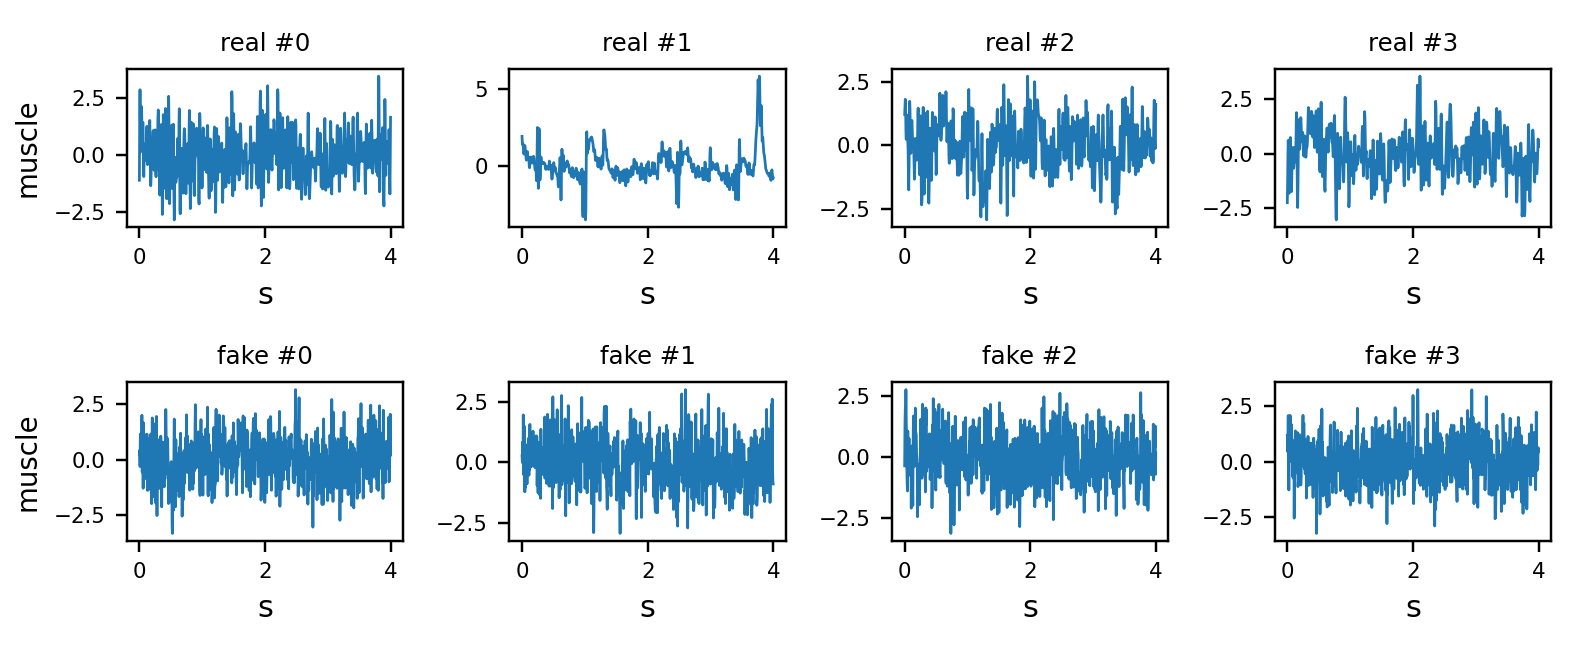
\includegraphics[width=\linewidth]{figs/muscle_realfake_panel.png}
  \caption{Qualitative \emph{muscle} windows: four real (top) and four synthetic (bottom).}
  \label{fig:qual-muscle}
\end{figure}

\subsection{Spectral fidelity}
We compare power spectral density (PSD) distributions between real and synthetic segments. For \emph{muscle}, Fig.~\ref{fig:psd-muscle} plots the median PSD with inter-quartile shading; synthetic traces exhibit a mild upward bias from $\sim$5–40\,Hz. Figure~\ref{fig:welch-by-artifact} summarizes Welch PSDs (channel-mean) across all artifacts, indicating broadly similar spectral envelopes with artifact-specific peaks.

\begin{figure}[t]
  \centering
  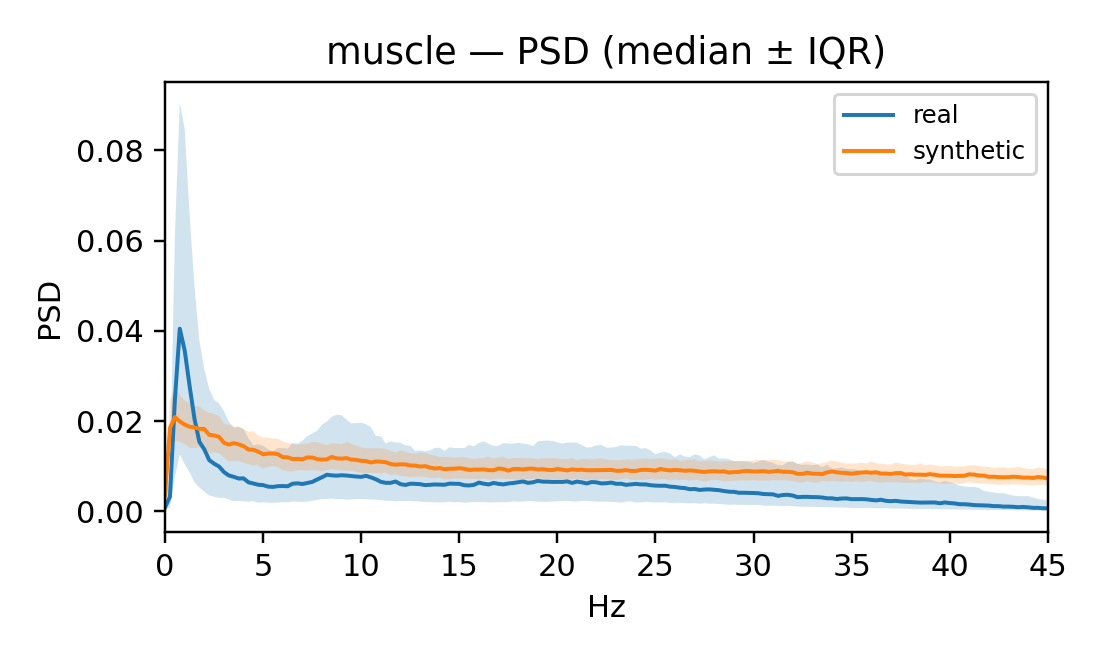
\includegraphics[width=0.78\linewidth]{figs/muscle_psd_median_iqr.png}
  \caption{\emph{Muscle} PSD (median $\pm$ IQR): synthetic slightly exceeds real across mid–high bands.}
  \label{fig:psd-muscle}
\end{figure}

\begin{figure}[t]
  \centering
  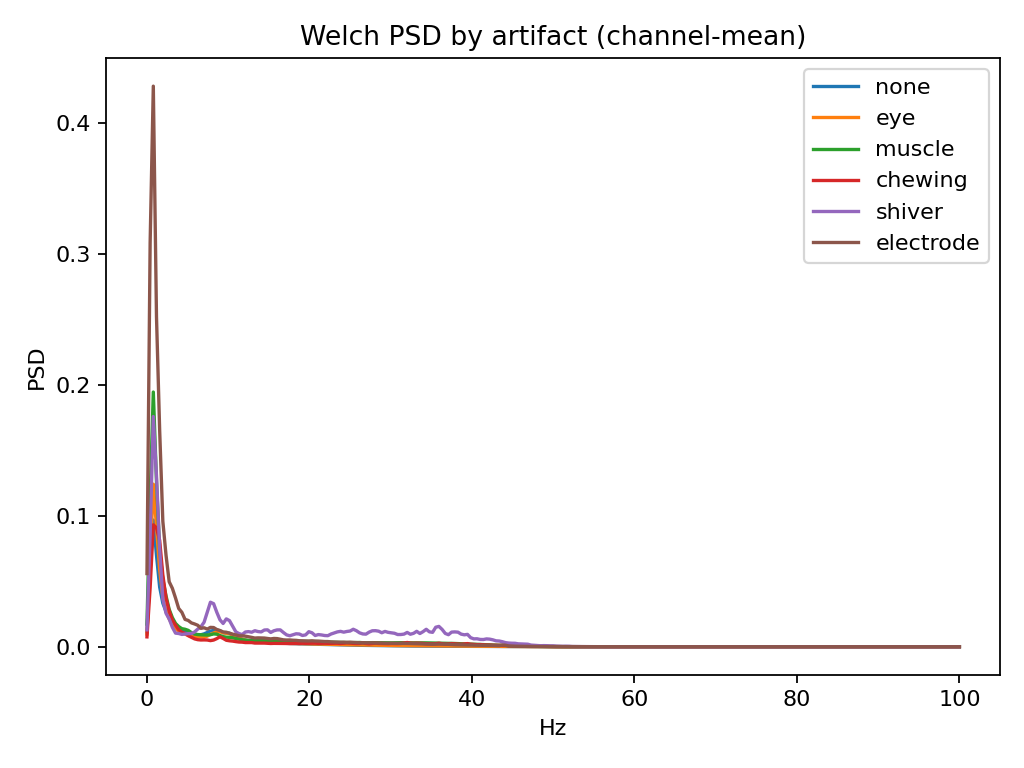
\includegraphics[width=0.85\linewidth]{figs/welch_psd_by_artifact.png}
  \caption{Welch PSD (channel-mean) by artifact on the held-out split.}
  \label{fig:welch-by-artifact}
\end{figure}

\subsection{Aggregate fidelity metrics}
Table~\ref{tab:fidelity} reports band-limited PSD deviations ($\Delta b$, lower is better), covariance Frobenius distance (Cov; lower is better), and ACF L2 discrepancy (lower is better). Values are comparable across artifacts, with slightly higher Cov/ACF for \emph{none}.

\begin{table}[t]
  \centering
  \caption{Fidelity metrics by artifact (lower is better). $\Delta b$ is absolute PSD deviation in band $b\!\in\!\{\delta,\theta,\alpha,\beta\}$.}
  \label{tab:fidelity}
  \vspace{0.25em}
  \small
  \begin{tabular}{lrrrrrrr}
    \toprule
    \textbf{Artifact} & $\mathbf{\Delta\delta}$ & $\mathbf{\Delta\theta}$ & $\mathbf{\Delta\alpha}$ & $\mathbf{\Delta\beta}$ & \textbf{Cov} $\downarrow$ & \textbf{ACF} $\downarrow$ & $\mathbf{n_{\text{fake}}}$ \\
    \midrule
    none       & 0.132 & 0.008 & 0.004 & 0.004 & 2.715 & 1.910 & 800 \\
    eye        & 0.131 & 0.008 & 0.004 & 0.004 & 2.702 & 1.900 & 800 \\
    muscle     & 0.131 & 0.008 & 0.004 & 0.004 & 2.705 & 1.903 & 800 \\
    chewing    & 0.131 & 0.007 & 0.004 & 0.004 & 2.712 & 1.901 & 800 \\
    shiver     & 0.131 & 0.007 & 0.003 & 0.004 & 2.694 & 1.907 & 800 \\
    electrode  & 0.131 & 0.007 & 0.004 & 0.004 & 2.719 & 1.901 & 800 \\
    \bottomrule
  \end{tabular}
\end{table}

\subsection{Two-sample diagnostics}
We quantify real–synthetic separability with a $1$-NN two-sample test (ideal $\approx 0.5$). Across artifacts, $1$-NN accuracy is $1.00$, indicating that a simple nearest-neighbor classifier perfectly separates real from synthetic in the chosen feature space; $k$NN precision/recall for synthetic are $0.00$, consistent with this gap. These diagnostics flag distribution mismatch despite moderate PSD/Cov/ACF alignment, and they localize future work (e.g., amplitude normalization, spectrum-aware loss/guidance, and artifact-condition calibration).

\paragraph{Summary.}
Qualitative waveforms are plausible and band-limited; spectra show mild synthetic over-power in mid–high bands, visible in \emph{muscle}. Aggregate PSD/Cov/ACF deviations are small but consistent across artifacts. However, two-sample tests indicate full separability (1-NN $=1.0$), suggesting that additional regularization or conditioning improvements are required to close the real–synthetic gap.


%%%%%%%%%%%%%%%%%%%%%%%%%%%%%%%%%%%%%%%%%%%%%%%%%%%%%%%%%%%%

\section{Discussion}

\subsection{Summary of Empirical Findings}
We investigated controllable EEG synthesis using a 1D U-Net with FiLM-style conditioning and a diffusion-based sampler. Across datasets derived from TUH (TUEG/TUAR), the model reproduced coarse morphology but exhibited systematic fidelity gaps in low-frequency bands (e.g., $\Delta\delta$ and $\Delta\theta$) and high Classifier Two-Sample Test (C2ST; 1-NN) separability. Concurrently, precision--recall for distributions (PRD) indicated low coverage of rare artifacts. Taken together, these signals suggest that while the generator captures broad spectral regularities, it under-covers the real distribution in clinically salient regimes \citep{lopezpaz2017c2st,sajjadi2018prd}.

\subsection{Methodological Contributions}
Two modeling choices proved effective. First, feature-wise linear modulation (FiLM) offered a lightweight and stable conditioning interface for artifact control with negligible sampling overhead \citep{perez2018film}. Second, domain-aligned metrics---Welch-PSD band deltas, channel covariance distance, and ACF $\ell_2$---provided interpretable diagnostics that track clinically meaningful deviations in power and correlation structure \citep{welch1967psd}. These metrics complemented task-space separability (C2ST) and distributional coverage (PRD) \citep{lopezpaz2017c2st,sajjadi2018prd}.

\subsection{Observed Failure Modes}
We consistently observed: (i) \emph{Under-coverage.} Near-zero PRD recall alongside high 1-NN accuracy indicates mode dropping despite visually plausible samples. (ii) \emph{Conditioning collapse.} Intended-match rates concentrated on specific artifact labels across runs, consistent with weak conditional gradients under aggressive noise schedules. (iii) \emph{Evaluation bias.} A recovery classifier trained on real data favored frequent artifacts, and global (non–class-stratified) recovery pools inflated measured separability.

\subsection{Remedial Strategies}
We propose three concrete interventions. \textbf{Strengthen conditioning:} increase FiLM width; inject class/timestep-aware adaptive normalization at multiple U-Net scales; and propagate class embeddings across down/up paths \citep{perez2018film}. \textbf{Schedule and sampler tuning:} adopt the cosine $\beta_t$ schedule \citep{nichol2021improved} and fewer denoising steps (DDIM) to preserve conditional signal; incorporate classifier-free guidance to trade fidelity and diversity at sampling time \citep{song2020ddim,ho2022cfg}. \textbf{Targeted reweighting and spectral consistency:} reweight losses by artifact frequency and oversample rare classes during the noising pipeline; add lightweight multi-resolution STFT losses to reduce observed band gaps without sacrificing diversity \citep{yamamoto2020parallelwavegan}.

\subsection{Validity and Limitations of Metrics}
C2ST is a sensitive shift detector but pessimistic if the representation is misaligned with clinically relevant structure \citep{lopezpaz2017c2st}. PRD is informative about precision--recall trade-offs yet depends on the embedding used to compute distances \citep{sajjadi2018prd}. EEG-specific metrics such as Welch-PSD deltas and covariance/ACF distances capture band-power and correlation differences but may miss cross-band phase relations or transient morphology. We therefore advocate reporting (i) raw-signal metrics (PSD/covariance/ACF), (ii) representation-space metrics (e.g., EEGNet embeddings) \citep{lawhern2018eegnet}, and (iii) task-grounded endpoints when augmentation is the goal.

\subsection{Dataset and External Validity Considerations}
Our training and evaluation relied on TUEG for scale and heterogeneity and TUAR for artifact supervision \citep{obeid2016tueg,hamid2020tuar}. Artifact taxonomies, montages, and acquisition protocols vary across institutions; thus, artifact-conditioned synthesis should be examined under cross-corpus transfer and with alternative montages. Emerging diffusion baselines for neurophysiological signals, including EEG and ECoG \citep{tosato2023eegdiffusion,vetter2024nddm}, provide natural anchors for external comparison.

\subsection{Ethical, Privacy, and Safety Considerations}
Diffusion models are not inherently privacy-preserving. Recent work demonstrates training-data extraction and membership inference against diffusion models \citep{carlini2023extracting,duan2023mia,matsumoto2023mia}, and unintended memorization remains a broader risk in generative models \citep{carlini2019secretsharer}. Prior to release, we recommend (i) de-duplication against training sets, (ii) exposure and membership-inference audits, and (iii) watermarking and mandatory labeling of synthetic artifacts when used downstream.


%%%%%%%%%%%%%%%%%%%%%%%%%%%%%%%%%%%%%%%%%%%%%%%%%%%%%%%%%%%%


\section{Future Work}

\subsection{Near-Term Enhancements: Conditioning, Recovery Pools, and Representation-Space Evaluation}
Immediate directions include multi-scale conditioning with classifier-free guidance and noise-dependent schedules, artifact-stratified recovery pools to mitigate overfitting to frequent perturbations, and evaluation in representation spaces (e.g., EEGNet embeddings) that are more sensitive to clinically salient morphology than pixel/pointwise metrics alone \citep{nichol2021improved,ho2022cfg,lawhern2018eegnet}. We will also explore spectral-consistency objectives (e.g., multi-resolution STFT losses) to stabilize conditional gradients in the waveform domain and reduce ringing/aliasing, alongside sampler/schedule co-design to control error accumulation under guidance \citep{yamamoto2020parallelwavegan,karras2022edm}.

\subsection{Architectural Generalization: Transformer Backbones and Flow-Based Alternatives}
While U-Net-style 1D backbones have been effective, replacing them with diffusion transformers adapted to sequences (patchified latent tokens with adaptive layer norm conditioning) may improve scaling and long-range temporal modeling \citep{peebles2023dit}. Beyond standard diffusion, we will evaluate \emph{flow-based} and \emph{consistency} alternatives that offer fewer sampling steps while retaining conditional controllability—specifically consistency models, rectified flows, and flow matching—assessing stability under strong guidance and the cost–quality trade-off for long 1D signals \citep{song2023consistency,liu2022rectifiedflow,lipman2022flowmatching}.

\subsection{Training Objectives and Sampler Design for Stable Guidance}
To reduce gradient variance and collapse under high guidance scales, we will combine (i) noise-/time-dependent guidance schedules with (ii) loss reweighting and preconditioning from the EDM design space, and (iii) distillation or consistency regularizers to compress iterative samplers into few-step generators without sacrificing conditional fidelity \citep{karras2022edm,nichol2021improved,salimans2022progressivedistill}. For audio-like biosignals, we will benchmark spectral objectives against waveform diffusion losses (e.g., DiffWave-style variants) and study their interaction with classifier-free guidance \citep{kong2020diffwave,ho2022cfg}.

\subsection{Conditioning Mechanisms Beyond Artifact Labels}
We will investigate structured conditioning that incorporates auxiliary channels and sensor geometry. Examples include ControlNet-style residual control branches for auxiliary biosignals (EOG/EMG) and spatial priors, and montage-aware embeddings (e.g., distance or graph-based encodings of electrode layouts) to improve cross-montage generalization \citep{zhang2023controlnet}. We will also study cross-dataset conditioning (domain tokens) to enable robust synthesis across heterogeneous clinical protocols.

\subsection{Evaluation Methodology: Representation- and Geometry-Aware Metrics}
Conventional sample quality/diversity proxies (e.g., PRD, C2ST) can be complemented with task-aligned distances computed in learned EEG representation spaces (SSL or task networks) and with geometry-aware statistics of second-order structure. We will therefore (i) adopt representation-based distances inspired by FAD for audio (instantiating an ``Fréchet EEG Distance'' with EEG encoders) and (ii) compare distribution gaps using kernel two-sample tests (MMD) over features; (iii) analyze cross-covariance geometry using Riemannian distances on SPD covariance manifolds to capture spatial patterns \citep{banville2021ssl,kilgour2019fad,gretton2012mmd,barachant2013riemannian}. These will be reported alongside downstream changes in AUROC/$F_1$ for seizure detection and artifact rejection.

\subsection{Clinical Validation and Multi-Institutional Benchmarking}
Beyond TUH-based artifacts and seizures, we will evaluate montage robustness and clinical utility across diverse cohorts (e.g., CHB-MIT), focusing on whether artifact-conditioned synthesis improves real endpoints: robust seizure detection under heavy contamination and reliable artifact rejection in preprocessing pipelines. Emphasis will be placed on \emph{downstream} metrics over proxy sample quality to ensure clinical relevance \citep{obeid2016tueg,goldberger2000physionet}.

\subsection{Data Governance, Privacy, and Provenance}
To reduce memorization risks during conditional synthesis, we will study differentially private training for diffusion/flow models and integrate provenance mechanisms (e.g., watermarking/fingerprinting adapted to 1D) to flag synthetic content in clinical workflows. Future work will quantify trade-offs among privacy budgets, conditional fidelity, and downstream task performance \citep{dockhorn2022dpdm,wen2023treering}.


%%%%%%%%%%%%%%%%%%%%%%%%%%%%%%%%%%%%%%%%%%%%%%%%%%%%%%%%%%%%

\newpage

\section{References}
\nocite{*}
\bibliographystyle{plain}
\bibliography{ConditionGen}


%%%%%%%%%%%%%%%%%%%%%%%%%%%%%%%%%%%%%%%%%%%%%%%%%%%%%%%%%%%%
\newpage
\appendix

\section{Appendices and Supplementary Material}


\subsection{Compute \& Environment}
\begin{itemize}
  \item \textbf{Machine:} Desktop workstation with NVIDIA RTX 4080 (16\,GB), 96\,GB RAM, 2\,TB SSD.
  \item \textbf{OS / Runtime:} Linux (Pop!\_OS 22.04 LTS), Python~3.x, PyTorch~2.x with CUDA~12.x.
  \item \textbf{Model:} 1D UNet with FiLM conditioning; widths $(64,128,256)$; conditioning dim $=13$.
  \item \textbf{Sampling config:} $80$ steps with classifier-free guidance scale $1.5$, EMA weights enabled, batch size $256$, $N{=}\,3000$ samples per artifact class.
  \item \textbf{Artifacts covered:} \texttt{none}, \texttt{eye}, \texttt{muscle}, \texttt{chewing}, \texttt{shiver}, \texttt{electrode}.
\end{itemize}

\subsection{Additional Figures}

\begin{figure}[t]
  \centering
  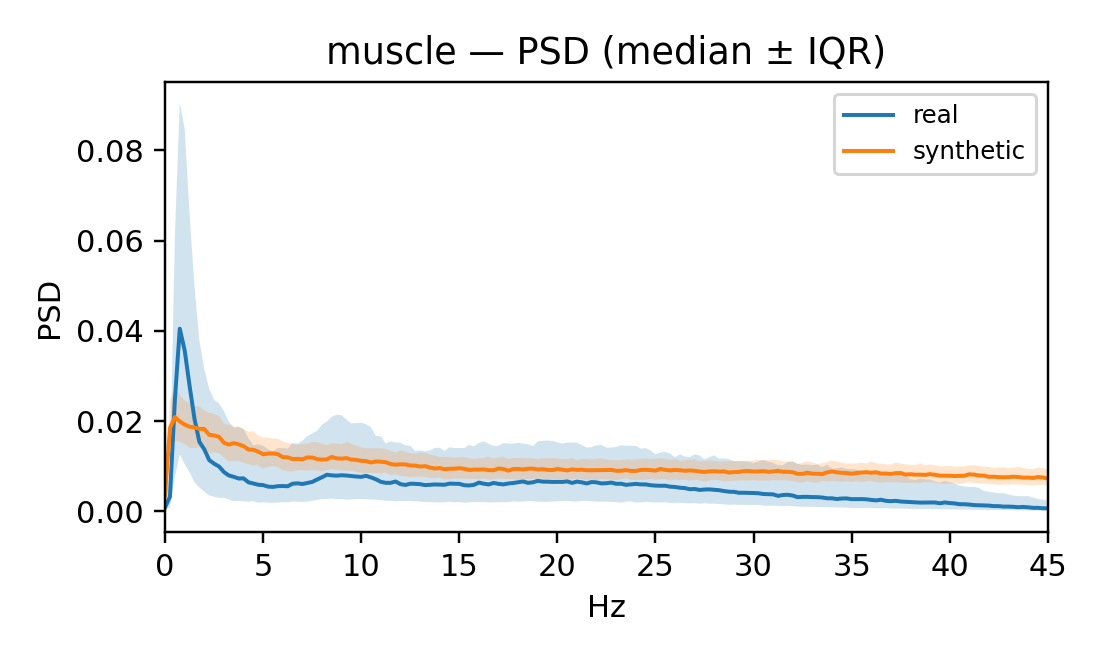
\includegraphics[width=0.9\linewidth]{figs/muscle_psd_median_iqr.png}
  \caption{\textbf{Muscle artifact:} Median power spectral density (PSD) with IQR bands for real vs.\ synthetic segments.}
  \label{fig:app-muscle-psd}
\end{figure}

\begin{figure}[t]
  \centering
  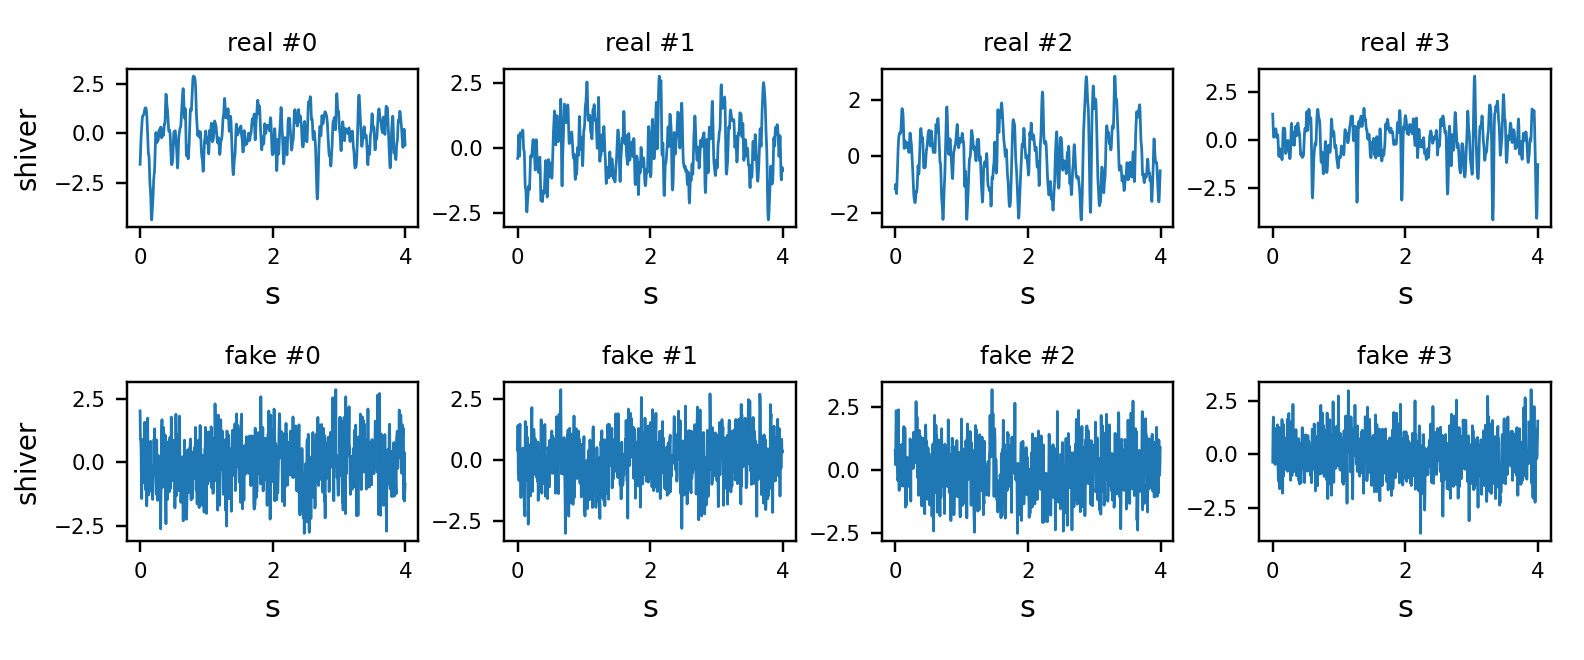
\includegraphics[width=0.95\linewidth]{figs/shiver_realfake_panel.png}
  \caption{\textbf{Shiver artifact:} Real/fake comparison panel illustrating representative time-domain windows and corresponding spectra.}
  \label{fig:app-shiver-panel}
\end{figure}

\begin{figure}[t]
  \centering
  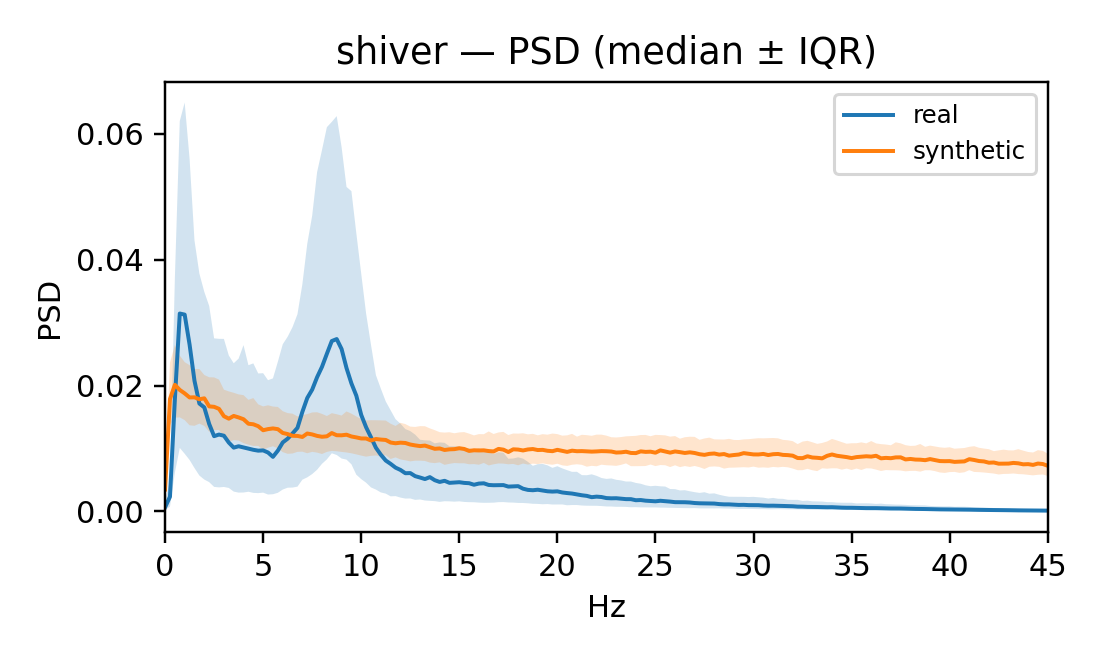
\includegraphics[width=0.9\linewidth]{figs/shiver_psd_median_iqr.png}
  \caption{\textbf{Shiver artifact:} Median PSD with IQR bands for real vs.\ synthetic segments.}
  \label{fig:app-shiver-psd}
\end{figure}

\newpage

%%%%%%%%%%%%%%%%%%%%%%%%%%%%%%%%%%%%%%%%%%%%%%%%%%%%%%%%%%%%

\clearpage
\section*{NeurIPS Paper Checklist}

\begin{enumerate}

\item {\bf Claims}
    \item[] Question: Do the main claims made in the abstract and introduction accurately reflect the paper's contributions and scope?
    \item[] Answer: \answerYes{}
    \item[] Justification: The abstract and introduction precisely state the method and the evaluation scope and they avoid broader clinical claims.
    \item[] Guidelines:
    \begin{itemize}
        \item The answer NA means that the abstract and introduction do not include the claims made in the paper.
        \item The abstract and/or introduction should clearly state the claims made, including the contributions made in the paper and important assumptions and limitations. A No or NA answer to this question will not be perceived well by the reviewers. 
        \item The claims made should match theoretical and experimental results, and reflect how much the results can be expected to generalize to other settings. 
        \item It is fine to include aspirational goals as motivation as long as it is clear that these goals are not attained by the paper. 
    \end{itemize}

\item {\bf Limitations}
    \item[] Question: Does the paper discuss the limitations of the work performed by the authors?
    \item[] Answer: \answerYes{}
    \item[] Justification: A dedicated Limitations paragraph notes dataset constraints (TUAR/TUEG only), potential covariate shift across sites/montages, limited ablations, and that downstream clinical utility is not established.
    \item[] Guidelines:
    \begin{itemize}
        \item The answer NA means that the paper has no limitation while the answer No means that the paper has limitations, but those are not discussed in the paper. 
        \item The authors are encouraged to create a separate "Limitations" section in their paper.
        \item The paper should point out any strong assumptions and how robust the results are to violations of these assumptions (e.g., independence assumptions, noiseless settings, model well-specification, asymptotic approximations only holding locally). The authors should reflect on how these assumptions might be violated in practice and what the implications would be.
        \item The authors should reflect on the scope of the claims made, e.g., if the approach was only tested on a few datasets or with a few runs. In general, empirical results often depend on implicit assumptions, which should be articulated.
        \item The authors should reflect on the factors that influence the performance of the approach. For example, a facial recognition algorithm may perform poorly when image resolution is low or images are taken in low lighting. Or a speech-to-text system might not be used reliably to provide closed captions for online lectures because it fails to handle technical jargon.
        \item The authors should discuss the computational efficiency of the proposed algorithms and how they scale with dataset size.
        \item If applicable, the authors should discuss possible limitations of their approach to address problems of privacy and fairness.
        \item While the authors might fear that complete honesty about limitations might be used by reviewers as grounds for rejection, a worse outcome might be that reviewers discover limitations that aren't acknowledged in the paper. The authors should use their best judgment and recognize that individual actions in favor of transparency play an important role in developing norms that preserve the integrity of the community. Reviewers will be specifically instructed to not penalize honesty concerning limitations.
    \end{itemize}

\item {\bf Theory assumptions and proofs}
    \item[] Question: For each theoretical result, does the paper provide the full set of assumptions and a complete (and correct) proof?
    \item[] Answer: \answerNA{}
    \item[] Justification: The paper is empirical and does not introduce new theorems or formal proofs; therefore no theoretical results or assumptions are claimed.
    \item[] Guidelines:
    \begin{itemize}
        \item The answer NA means that the paper does not include theoretical results. 
        \item All the theorems, formulas, and proofs in the paper should be numbered and cross-referenced.
        \item All assumptions should be clearly stated or referenced in the statement of any theorems.
        \item The proofs can either appear in the main paper or the supplemental material, but if they appear in the supplemental material, the authors are encouraged to provide a short proof sketch to provide intuition. 
        \item Inversely, any informal proof provided in the core of the paper should be complemented by formal proofs provided in appendix or supplemental material.
        \item Theorems and Lemmas that the proof relies upon should be properly referenced. 
    \end{itemize}

    \item {\bf Experimental result reproducibility}
    \item[] Question: Does the paper fully disclose all the information needed to reproduce the main experimental results of the paper to the extent that it affects the main claims and/or conclusions of the paper (regardless of whether the code and data are provided or not)?
    \item[] Answer: \answerYes{}
    \item[] Justification: We specify datasets, preprocessing, splits, model architecture, conditioning, loss/schedules, samplers, hyperparameters, seeds where applicable, and provide end-to-end commands in the supplement to reproduce figures and tables.
    \item[] Guidelines:
    \begin{itemize}
        \item The answer NA means that the paper does not include experiments.
        \item If the paper includes experiments, a No answer to this question will not be perceived well by the reviewers: Making the paper reproducible is important, regardless of whether the code and data are provided or not.
        \item If the contribution is a dataset and/or model, the authors should describe the steps taken to make their results reproducible or verifiable. 
        \item Depending on the contribution, reproducibility can be accomplished in various ways. For example, if the contribution is a novel architecture, describing the architecture fully might suffice, or if the contribution is a specific model and empirical evaluation, it may be necessary to either make it possible for others to replicate the model with the same dataset, or provide access to the model. In general. releasing code and data is often one good way to accomplish this, but reproducibility can also be provided via detailed instructions for how to replicate the results, access to a hosted model (e.g., in the case of a large language model), releasing of a model checkpoint, or other means that are appropriate to the research performed.
        \item While NeurIPS does not require releasing code, the conference does require all submissions to provide some reasonable avenue for reproducibility, which may depend on the nature of the contribution. For example
        \begin{enumerate}
            \item If the contribution is primarily a new algorithm, the paper should make it clear how to reproduce that algorithm.
            \item If the contribution is primarily a new model architecture, the paper should describe the architecture clearly and fully.
            \item If the contribution is a new model (e.g., a large language model), then there should either be a way to access this model for reproducing the results or a way to reproduce the model (e.g., with an open-source dataset or instructions for how to construct the dataset).
            \item We recognize that reproducibility may be tricky in some cases, in which case authors are welcome to describe the particular way they provide for reproducibility. In the case of closed-source models, it may be that access to the model is limited in some way (e.g., to registered users), but it should be possible for other researchers to have some path to reproducing or verifying the results.
        \end{enumerate}
    \end{itemize}


\item {\bf Open access to data and code}
    \item[] Question: Does the paper provide open access to the data and code, with sufficient instructions to faithfully reproduce the main experimental results, as described in supplemental material?
    \item[] Answer: \answerYes{}
    \item[] Justification: Data is public (TUAR/TUEG) and paper contains pointers and preparation steps so others can recreate our pipelines.
    \item[] Guidelines:
    \begin{itemize}
        \item The answer NA means that paper does not include experiments requiring code.
        \item Please see the NeurIPS code and data submission guidelines (\url{https://nips.cc/public/guides/CodeSubmissionPolicy}) for more details.
        \item While we encourage the release of code and data, we understand that this might not be possible, so “No” is an acceptable answer. Papers cannot be rejected simply for not including code, unless this is central to the contribution (e.g., for a new open-source benchmark).
        \item The instructions should contain the exact command and environment needed to run to reproduce the results. See the NeurIPS code and data submission guidelines (\url{https://nips.cc/public/guides/CodeSubmissionPolicy}) for more details.
        \item The authors should provide instructions on data access and preparation, including how to access the raw data, preprocessed data, intermediate data, and generated data, etc.
        \item The authors should provide scripts to reproduce all experimental results for the new proposed method and baselines. If only a subset of experiments are reproducible, they should state which ones are omitted from the script and why.
        \item At submission time, to preserve anonymity, the authors should release anonymized versions (if applicable).
        \item Providing as much information as possible in supplemental material (appended to the paper) is recommended, but including URLs to data and code is permitted.
    \end{itemize}


\item {\bf Experimental setting/details}
    \item[] Question: Does the paper specify all the training and test details (e.g., data splits, hyperparameters, how they were chosen, type of optimizer, etc.) necessary to understand the results?
    \item[] Answer: \answerYes{}
    \item[] Justification: The Methods and Appendix enumerate data splits, montage, sampling rate, optimizer/schedule, diffusion steps/sampler, batch size, conditioning scheme, and selection rationales.
    \item[] Guidelines:
    \begin{itemize}
        \item The answer NA means that the paper does not include experiments.
        \item The experimental setting should be presented in the core of the paper to a level of detail that is necessary to appreciate the results and make sense of them.
        \item The full details can be provided either with the code, in appendix, or as supplemental material.
    \end{itemize}

\item {\bf Experiment statistical significance}
    \item[] Question: Does the paper report error bars suitably and correctly defined or other appropriate information about the statistical significance of the experiments?
    \item[] Answer: \answerNo{}
    \item[] Justification: Current results report point estimates across runs/partitions without CIs; we note this and plan to include bootstrap CIs and seed variance in a revision.
    \item[] Guidelines:
    \begin{itemize}
        \item The answer NA means that the paper does not include experiments.
        \item The authors should answer "Yes" if the results are accompanied by error bars, confidence intervals, or statistical significance tests, at least for the experiments that support the main claims of the paper.
        \item The factors of variability that the error bars are capturing should be clearly stated (for example, train/test split, initialization, random drawing of some parameter, or overall run with given experimental conditions).
        \item The method for calculating the error bars should be explained (closed form formula, call to a library function, bootstrap, etc.)
        \item The assumptions made should be given (e.g., Normally distributed errors).
        \item It should be clear whether the error bar is the standard deviation or the standard error of the mean.
        \item It is OK to report 1-sigma error bars, but one should state it. The authors should preferably report a 2-sigma error bar than state that they have a 96\% CI, if the hypothesis of Normality of errors is not verified.
        \item For asymmetric distributions, the authors should be careful not to show in tables or figures symmetric error bars that would yield results that are out of range (e.g. negative error rates).
        \item If error bars are reported in tables or plots, The authors should explain in the text how they were calculated and reference the corresponding figures or tables in the text.
    \end{itemize}

\item {\bf Experiments compute resources}
    \item[] Question: For each experiment, does the paper provide sufficient information on the computer resources (type of compute workers, memory, time of execution) needed to reproduce the experiments?
    \item[] Answer: \answerYes{}
    \item[] Justification: Appendix provides environment details
    \item[] Guidelines:
    \begin{itemize}
        \item The answer NA means that the paper does not include experiments.
        \item The paper should indicate the type of compute workers CPU or GPU, internal cluster, or cloud provider, including relevant memory and storage.
        \item The paper should provide the amount of compute required for each of the individual experimental runs as well as estimate the total compute. 
        \item The paper should disclose whether the full research project required more compute than the experiments reported in the paper (e.g., preliminary or failed experiments that didn't make it into the paper). 
    \end{itemize}
    
\item {\bf Code of ethics}
    \item[] Question: Does the research conducted in the paper conform, in every respect, with the NeurIPS Code of Ethics \url{https://neurips.cc/public/EthicsGuidelines}?
    \item[] Answer: \answerYes{}
    \item[] Justification: We use de-identified, publicly available EEG datasets under their licenses.
    \item[] Guidelines:
    \begin{itemize}
        \item The answer NA means that the authors have not reviewed the NeurIPS Code of Ethics.
        \item If the authors answer No, they should explain the special circumstances that require a deviation from the Code of Ethics.
        \item The authors should make sure to preserve anonymity (e.g., if there is a special consideration due to laws or regulations in their jurisdiction).
    \end{itemize}


\item {\bf Broader impacts}
    \item[] Question: Does the paper discuss both potential positive societal impacts and negative societal impacts of the work performed?
    \item[] Answer: \answerYes{}
    \item[] Justification: We outline benefits and risks with mitigation notes.
    \item[] Guidelines:
    \begin{itemize}
        \item The answer NA means that there is no societal impact of the work performed.
        \item If the authors answer NA or No, they should explain why their work has no societal impact or why the paper does not address societal impact.
        \item Examples of negative societal impacts include potential malicious or unintended uses (e.g., disinformation, generating fake profiles, surveillance), fairness considerations (e.g., deployment of technologies that could make decisions that unfairly impact specific groups), privacy considerations, and security considerations.
        \item The conference expects that many papers will be foundational research and not tied to particular applications, let alone deployments. However, if there is a direct path to any negative applications, the authors should point it out. For example, it is legitimate to point out that an improvement in the quality of generative models could be used to generate deepfakes for disinformation. On the other hand, it is not needed to point out that a generic algorithm for optimizing neural networks could enable people to train models that generate Deepfakes faster.
        \item The authors should consider possible harms that could arise when the technology is being used as intended and functioning correctly, harms that could arise when the technology is being used as intended but gives incorrect results, and harms following from (intentional or unintentional) misuse of the technology.
        \item If there are negative societal impacts, the authors could also discuss possible mitigation strategies (e.g., gated release of models, providing defenses in addition to attacks, mechanisms for monitoring misuse, mechanisms to monitor how a system learns from feedback over time, improving the efficiency and accessibility of ML).
    \end{itemize}
    
\item {\bf Safeguards}
    \item[] Question: Does the paper describe safeguards that have been put in place for responsible release of data or models that have a high risk for misuse (e.g., pretrained language models, image generators, or scraped datasets)?
    \item[] Answer: \answerNA{}
    \item[] Justification: The released assets (training code and small domain-specific models) are not high-risk general-purpose generators; we nevertheless include usage notes and disclaimers but no gated access is required.
    \item[] Guidelines:
    \begin{itemize}
        \item The answer NA means that the paper poses no such risks.
        \item Released models that have a high risk for misuse or dual-use should be released with necessary safeguards to allow for controlled use of the model, for example by requiring that users adhere to usage guidelines or restrictions to access the model or implementing safety filters. 
        \item Datasets that have been scraped from the Internet could pose safety risks. The authors should describe how they avoided releasing unsafe images.
        \item We recognize that providing effective safeguards is challenging, and many papers do not require this, but we encourage authors to take this into account and make a best faith effort.
    \end{itemize}

\item {\bf Licenses for existing assets}
    \item[] Question: Are the creators or original owners of assets (e.g., code, data, models), used in the paper, properly credited and are the license and terms of use explicitly mentioned and properly respected?
    \item[] Answer: \answerYes{}
    \item[] Justification: We cite the data sources used as well as the packages.
    \item[] Guidelines:
    \begin{itemize}
        \item The answer NA means that the paper does not use existing assets.
        \item The authors should cite the original paper that produced the code package or dataset.
        \item The authors should state which version of the asset is used and, if possible, include a URL.
        \item The name of the license (e.g., CC-BY 4.0) should be included for each asset.
        \item For scraped data from a particular source (e.g., website), the copyright and terms of service of that source should be provided.
        \item If assets are released, the license, copyright information, and terms of use in the package should be provided. For popular datasets, \url{paperswithcode.com/datasets} has curated licenses for some datasets. Their licensing guide can help determine the license of a dataset.
        \item For existing datasets that are re-packaged, both the original license and the license of the derived asset (if it has changed) should be provided.
        \item If this information is not available online, the authors are encouraged to reach out to the asset's creators.
    \end{itemize}

\item {\bf New assets}
    \item[] Question: Are new assets introduced in the paper well documented and is the documentation provided alongside the assets?
    \item[] Answer: \answerNA{}.
    \item[] Justification: Did not provide any additional code apart from the instructions given.
    \item[] Guidelines:
    \begin{itemize}
        \item The answer NA means that the paper does not release new assets.
        \item Researchers should communicate the details of the dataset/code/model as part of their submissions via structured templates. This includes details about training, license, limitations, etc. 
        \item The paper should discuss whether and how consent was obtained from people whose asset is used.
        \item At submission time, remember to anonymize your assets (if applicable). You can either create an anonymized URL or include an anonymized zip file.
    \end{itemize}

\item {\bf Crowdsourcing and research with human subjects}
    \item[] Question: For crowdsourcing experiments and research with human subjects, does the paper include the full text of instructions given to participants and screenshots, if applicable, as well as details about compensation (if any)? 
    \item[] Answer: \answerNA{}.
    \item[] Justification: No new human-subjects data or crowdsourcing were conducted; we rely solely on public de-identified datasets.
    \item[] Guidelines:
    \begin{itemize}
        \item The answer NA means that the paper does not involve crowdsourcing nor research with human subjects.
        \item Including this information in the supplemental material is fine, but if the main contribution of the paper involves human subjects, then as much detail as possible should be included in the main paper. 
        \item According to the NeurIPS Code of Ethics, workers involved in data collection, curation, or other labor should be paid at least the minimum wage in the country of the data collector. 
    \end{itemize}

\item {\bf Institutional review board (IRB) approvals or equivalent for research with human subjects}
    \item[] Question: Does the paper describe potential risks incurred by study participants, whether such risks were disclosed to the subjects, and whether Institutional Review Board (IRB) approvals (or an equivalent approval/review based on the requirements of your country or institution) were obtained?
    \item[] Answer: \answerNA{}
    \item[] Justification: The work analyzes public, de-identified EEG datasets and does not involve direct human-subjects research requiring IRB review for this study.
    \item[] Guidelines:
    \begin{itemize}
        \item The answer NA means that the paper does not involve crowdsourcing nor research with human subjects.
        \item Depending on the country in which research is conducted, IRB approval (or equivalent) may be required for any human subjects research. If you obtained IRB approval, you should clearly state this in the paper. 
        \item We recognize that the procedures for this may vary significantly between institutions and locations, and we expect authors to adhere to the NeurIPS Code of Ethics and the guidelines for their institution. 
        \item For initial submissions, do not include any information that would break anonymity (if applicable), such as the institution conducting the review.
    \end{itemize}

\item {\bf Declaration of LLM usage}
    \item[] Question: Does the paper describe the usage of LLMs if it is an important, original, or non-standard component of the core methods in this research? Note that if the LLM is used only for writing, editing, or formatting purposes and does not impact the core methodology, scientific rigorousness, or originality of the research, declaration is not required.
    %this research? 
    \item[] Answer: \answerNA{}
    \item[] Justification: LLMs are not part of the core technical method; any editorial assistance does not impact the scientific methodology and thus does not require declaration.
    \item[] Guidelines:
    \begin{itemize}
        \item The answer NA means that the core method development in this research does not involve LLMs as any important, original, or non-standard components.
        \item Please refer to our LLM policy (\url{https://neurips.cc/Conferences/2025/LLM}) for what should or should not be described.
    \end{itemize}

\end{enumerate}

\end{document}